% def.tex

% File containing LaTeX macros.
% Has grown by accretion; can be better organized.

\documentclass{article}
\usepackage{amsmath}
\usepackage{amssymb}
\usepackage{bm}
\usepackage{graphicx}
\usepackage{epstopdf}
\DeclareGraphicsRule{.tif}{png}{.png}{`convert #1 `basename #1 .tif`.png}
\usepackage{color}
\usepackage{pdfsync}
\pagestyle{plain}

%\pagestyle{empty}

\textheight 9 true in
\textwidth 6.5 true in
\hoffset -.75 true in
\voffset -.75 true in
 \mathsurround=2pt  \parskip=2pt
\def\crv{\cr\noalign{\vskip7pt}} 

\def\a{\alpha } \def\b{\beta } \def\d{\delta } \def\D{\Delta } \def\e{\epsilon }
\def\g{\gamma } \def\G{\Gamma} \def\k{\kappa} \def\l{\lambda } \def\L{\Lambda }
\def\th{\theta } \def\Th{\Theta} \def\r{\rho} \def\o{\omega} \def\O{\Omega}
\def\ve{\varepsilon} 

\def\sA{{\cal A}} \def\sB{{\cal B}} \def\sC{{\cal C}} \def\sE{{\cal E}} \def\sI{{\cal I}}
\def\sR{{\cal R}} \def\sF{{\cal F}} \def\sG{{\cal G}} \def\sM{{\cal M}}
\def\sT{{\cal T}} \def\sH{{\cal H}} \def\sD{{\cal D}} \def\sW{{\cal W}}
\def\sL{{\cal L}} \def\sP{{\cal P}} \def\s{\sigma } \def\S{\Sigma}
\def\sU{{\cal U}} \def\sY{{\cal Y}}

\def\gm{\gamma -1}
\def\summ{\sum_{j=1}^4}

\def\bb{{\bm b}} \def\yb{{\bm y}}
\def\ub{{\bm u}}  \def\xb{{\bm x}} \def\vb{{\bm v}} \def\wb{{\bm w}}
\def\omegab{{\bm \omega}} \def\rb{{\bm r}} \def\ib{{\bm i}} \def\jb{{\bm j}}
\def\lb{{\bm l}} \def\kb{{\bm k}} \def\Ab{{\bm A}} \def\fb{{\bm f}} \def\Ub{{\bm U}}
\def\Fb{{\bm F}} \def\nb{{\bm n}} \def\Db{{\bm D}} \def\eb{{\bm e}}
\def\gb{{\bm g}}  \def\hb{{\bm h}} \def\Yb{{\bm Y}} \def\Rb{{\bm R}} 

\def\As1{{\bf {\cal A}}_1}\def\DO{{\cal D}_0} \def\UO{{\cal U}_0}
\def\ie{{\it{i.e.}}}

\def\ubbar{{\bf {\bar{u}}}} \def\sbar{{\bar{\sigma }}} \def\ubar{{\bar{u}}}  
\def\abar{{\bar{a}}} \def\vbar{{\bar{v}}}  \def\rbar{{\bar{\rho}}}
\def\pbar{{\bar{p}}} \def\ebar{{\bar{e}}} \def\Tbar{{\bar{T}}}
\def\bbar{{\bar{\beta}}} \def\Mbar{{\bar{M}}}  \def \sMbar{{\bar{\cal M}}}
\def\Ebar{{\bar{E}}} \def\sMbar{{\bar{\cal M}}}
\def\sPbar{{\bar{\cal P}}} \def\xbar{{\bar{x}}}

\newcommand{\pdv}[2]{\frac{\partial#1}{\partial#2}}
\newcommand{\dv}[2]{\frac{d#1}{d#2}}
\newcommand{\ord}[2]{#1^{(#2)}}
\newcommand{\vct}[1]{\vec{#1}}

 \newcommand{\bc}{\begin{center}}
 \newcommand{\ec}{\end{center}}
 
 \newcommand{\bq}{\begin{equation}}
 \newcommand{\eq}{\end{equation}}
 
 \newcommand{\beqs}{\begin{eqnarray}}
 \newcommand{\eeqs}{\end{eqnarray}}
 
 \newcommand{\beqa}{\begin{eqnarray*}}
 \newcommand{\eeqa}{\end{eqnarray*}}
 
 \newcommand{\ol}{\overline}
 \newcommand{\ul}{\underline}
 
 \newcommand{\dint}{{\int \!\! \int \!\!}}
 \newcommand{\tint}{{\int \!\! \int \!\! \int \!\!}}
 
 \newcommand{\bfig}{\begin{figure}}
 \newcommand{\efig}{\end{figure}}
 
 \newcommand{\cen}{\centering}
 \newcommand{\n}{\noindent}
 
 \newcommand{\btab}{\begin{table}}
 \newcommand{\etab}{\end{table}}
 
 \newcommand{\btbl}{\begin{tabular}}
 \newcommand{\etbl}{\end{tabular}}
 
 \newcommand{\bdes}{\begin{description}}
 \newcommand{\edes}{\end{description}}
 
 \newcommand{\benum}{\begin{enumerate}}
 \newcommand{\eenum}{\end{enumerate}}
 
 \newcommand{\bite}{\begin{itemize}}
 \newcommand{\eite}{\end{itemize}}
 
 \newcommand{\cle}{\clearpage}
 \newcommand{\npg}{\newpage}
 
 \newcommand{\bss}{\begin{singlespace}}
 \newcommand{\ess}{\end{singlespace}}
 
 \newcommand{\bhalf}{\begin{onehalfspace}}
 \newcommand{\ehalf}{\end{onehalfspace}}
 
 \newcommand{\bds}{\begin{doublespace}}
 \newcommand{\eds}{\end{doublespace}}
 
 \newcommand{\eps}{\mbox{$\epsilon$}} 
 \newcommand{\stilde}{\mbox{$\tilde s$}} 
 \newcommand{\shat}{\mbox{$\hat s$}} 

 \newcommand{\blue}{\color{blue}}
 \newcommand{\red}{\color{red}}
 \newcommand{\magenta}{\color{magenta}}
 \newcommand{\green}{\color{green}}
 \newcommand{\nc}{\normalcolor}



\def\arg{{\rm{arg}}}
\def\Arg{{\rm{Arg}}}
\def\imath{i}
\def\Log{{\rm{Log}}}
\def\erfc{{\rm{erfc}}}
\def\Oh{\mathcal{O}}
\def\oh{\mathsf{o}}

\def\Res{{\rm{Res}}}

\def\fl{{\rm{fl}}}

\def\Xint#1{\mathchoice
{\XXint\displaystyle\textstyle{#1}}%
{\XXint\textstyle\scriptstyle{#1}}%
{\XXint\scriptstyle\scriptscriptstyle{#1}}%
{\XXint\scriptscriptstyle\scriptscriptstyle{#1}}%
\!\int}
\def\XXint#1#2#3{{\setbox0=\hbox{$#1{#2#3}{\int}$ }
\vcenter{\hbox{$#2#3$ }}\kern-.6\wd0}}
\def\ddashint{\Xint=}
\def\dashint{\Xint-}

%\numberwithin{equation}{section}
\pagestyle{empty}
\begin{document}
Wang xinshi 661975305
\begin{center}
\large{ MATH-2400 \hspace{.25in}  INTRODUCTION TO DIFFERENTIAL EQUATIONS \hspace{.25in}SPRING 2021\\ Homework-4   \\ Assigned Friday Feb 19, 2021 \\ Due 12:00 Noon, Friday Feb 26, 2021}\end{center}

\bigskip
\n\ul{NOTES}
\benum
\item 
Practice problems listed below and taken from the textbook are for your own practice, and are not to be turned in.
\item 
Legible, handwritten solutions will be acceptable, but the use of a typesetting system such as LaTeX is strongly recommended.  \blue{\bf Do not turn in your rough attempt at solving a problem; once you have worked out the solution, copy it neatly or typeset it before submission, after removing all false starts.}\nc
\item 
Please write your solutions clearly and coherently, with the work displayed in a sequential manner and sufficient explanation provided so that your strategy and approach are transparent to the reader. 
\item 
Figures, if any, should be neatly drawn by hand, properly labelled and captioned.  
\item 
The assignment is to be submitted electronically to LMS  as a single pdf file.  Be sure that the pages are properly oriented and well lighted.  \blue{\bf Please do not e-mail your homework submission to the TAs or the instructors.}\nc
\eenum

\bigskip


\bc {\bf Practice Problems from the textbook (not to be turned in)} \ec

\n Exercises from Chapter 3, page 51: 3j, 4(h,i,j), 5(a,d,g,f), 6(a,c), 7.

\medskip

\bc {\bf Subjective part: problems to be turned in} \ec

\begin{enumerate}

% Problem 1
\item (20 points) Solve the following initial-value problems.
\benum
\item 
$y''-2y'-8y=0, \quad y(0)=6, \; y'(0)=6.$

Let $y = e^{rt}$, then we have $$y'' = r^2e^{rt}$$ $$y' = re^{rt}$$  $$y = e^{rt}$$

Substitute those values into the original DE gives us the characteristic equation: $$(r^2-2r-8)e^{rt} = 0$$

We can factor the equation into $(r-4)(r+2) = 0$, which gives us $r = 4$ and $r = -2$. Therefore we have $y_1(t) = e^{4t}$ and $y_2(t) = e^{-2t}$. Combining those two gives us $$y(t) = C_1e^{4t}+C_2e^{-2t}$$

After taking the derivative, we have $$y'(t) = 4C_1e^{-4t}-2C_2e^{2t}$$

Substituting the IC in, we have 
\begin{equation*}
	\begin{cases}
		C_1+C_2 &= 6\\
		4C_1 - 2C_2 &= 6
	\end{cases}
\end{equation*}

Thus we have $C_1 = 3$ and $C_2 = 3$. Thus the solution is $y(t) = 3e^{4t}+3e^{-2t}$.

\item 
$25y''-30y'+9y=0, \quad y(0)=5, \; y'(0)=-5.$
\eenum

Let $y = e^{rt}$, then we have $$y'' = r^2e^{rt}$$ $$y' = re^{rt}$$  $$y = e^{rt}$$

Substitute those values into the original DE gives us the characteristic equation: $$(25r^2-30r+9)e^{rt} = 0$$

From the characteristic formula we have $r = \dfrac{-b \pm \sqrt{b^2 - 4ac}}{2a}=\dfrac{3}{5}$. Therefore the general solution directly from the \textbf{Remark} section in lecture 06: $$y(t) = C_1e^{\dfrac{3}{5}t}+C_2te^{\dfrac{3}{5}t}$$  
After taking the derivative, we have $$y'(t) = \dfrac{3}{5}C_1e^{\dfrac{3}{5}t}+C_2e^{\dfrac{3}{5}t}+\dfrac{3}{5}C_2te^{\dfrac{3}{5}t}$$


Substituting the IC in, we have 
\begin{equation*}
	\begin{cases}
		C_1 &= 5\\
		\dfrac{3}{5}C_1 + C_2 &= -5
	\end{cases}
\end{equation*}

Thus we have $C_1 = 5$ and $C_2 = -8$. Thus the solution is $y(t) = 5e^{\dfrac{3}{5}t}-8te^{\dfrac{3}{5}t}$.

%Problem 2
\item (20 points)  Find the solution of the IVP
\begin{equation*}
y''-2y'+17y=0, \quad y(0)=\frac{3}{2}, \; y'(0)=\frac{3}{2} + 6\sqrt 3.
\end{equation*}
Express your answer in the each of the two forms discussed in class.  Draw a rough sketch of the solution on a properly labelled graph.\\

\noindent \textbf{Approach 1.}\\
Let $y = e^{rt}$, then we have $$y'' = r^2e^{rt}$$ $$y' = re^{rt}$$  $$y = e^{rt}$$

Substitute those values into the original DE gives us the characteristic equation: $$(r^2-2r+17)e^{rt} = 0$$

From the characteristic formula we have $r = \dfrac{-b \pm \sqrt{b^2 - 4ac}}{2a}=\dfrac{2 \pm \sqrt{4-68}}{2} = 1 \pm 4i$.\\
For $r = 1 + 4i$ the complex solution is 
$$Y_1(t) = e^{(1+4i)t}=e^{t}cos(4t)+ie^{t}sin(4t)$$

We can find the fundamental set of solutions $$y_1(t) = e^tcos4t$$ $$y_2(t) = e^tsin4t$$

Therefore the general solution is $$y(t) = C_1e^tcos(4t)+ C_2e^tsin(4t)$$

The derivative is $$y'(t) = C_1[e^tcos(4t)-4e^tsin(4t)]+C_2[e^tsin(4t)+4e^tcos(4t)]$$
Substituting the IC in, we have 
\begin{equation*}
	\begin{cases}
		C_1 &= \dfrac{3}{2}\\
		\\
		C_1 + 4C_2 &= \dfrac{3}{2}+6\sqrt{3}\\
	\end{cases}
\end{equation*}

Thus we have $C_1 = \dfrac{3}{2}$ and $C_2 = \dfrac{3 \sqrt{3}}{2}$. Thus the solution is $y(t) = \dfrac{3}{2}e^tcos(4t)+ \dfrac{3 \sqrt{3}}{2}e^tsin(4t)$.\\

\textbf{Approach 2.}
\begin{equation*}
	\begin{cases}
		R cos \phi &= \dfrac{3}{2}\\
		\\
		R sin \phi &= \dfrac{3 \sqrt{3}}{2}\\
	\end{cases}
\end{equation*}

Squaring the equations we have $$R^2 = (\dfrac{3}{2})^2 + (\dfrac{3 \sqrt{3}}{2})^2 = \dfrac{9}{16}$$
Thus $R = \dfrac{3}{4}$
We also have $$tan \phi = \sqrt{3}$$

There is no doubt that $\phi \in (0, 2 \pi)$. Since $R cos \phi > 0$, $R sin \phi >0$, and $R > 0$, $\phi \in (0, \dfrac{\pi}{2})$. Therefore $\phi = \dfrac{\pi}{3}$

Therefore we have the following solution: $y(t) = \dfrac{3}{4}e^tcos(4t - \dfrac{\pi}{4})$\\
	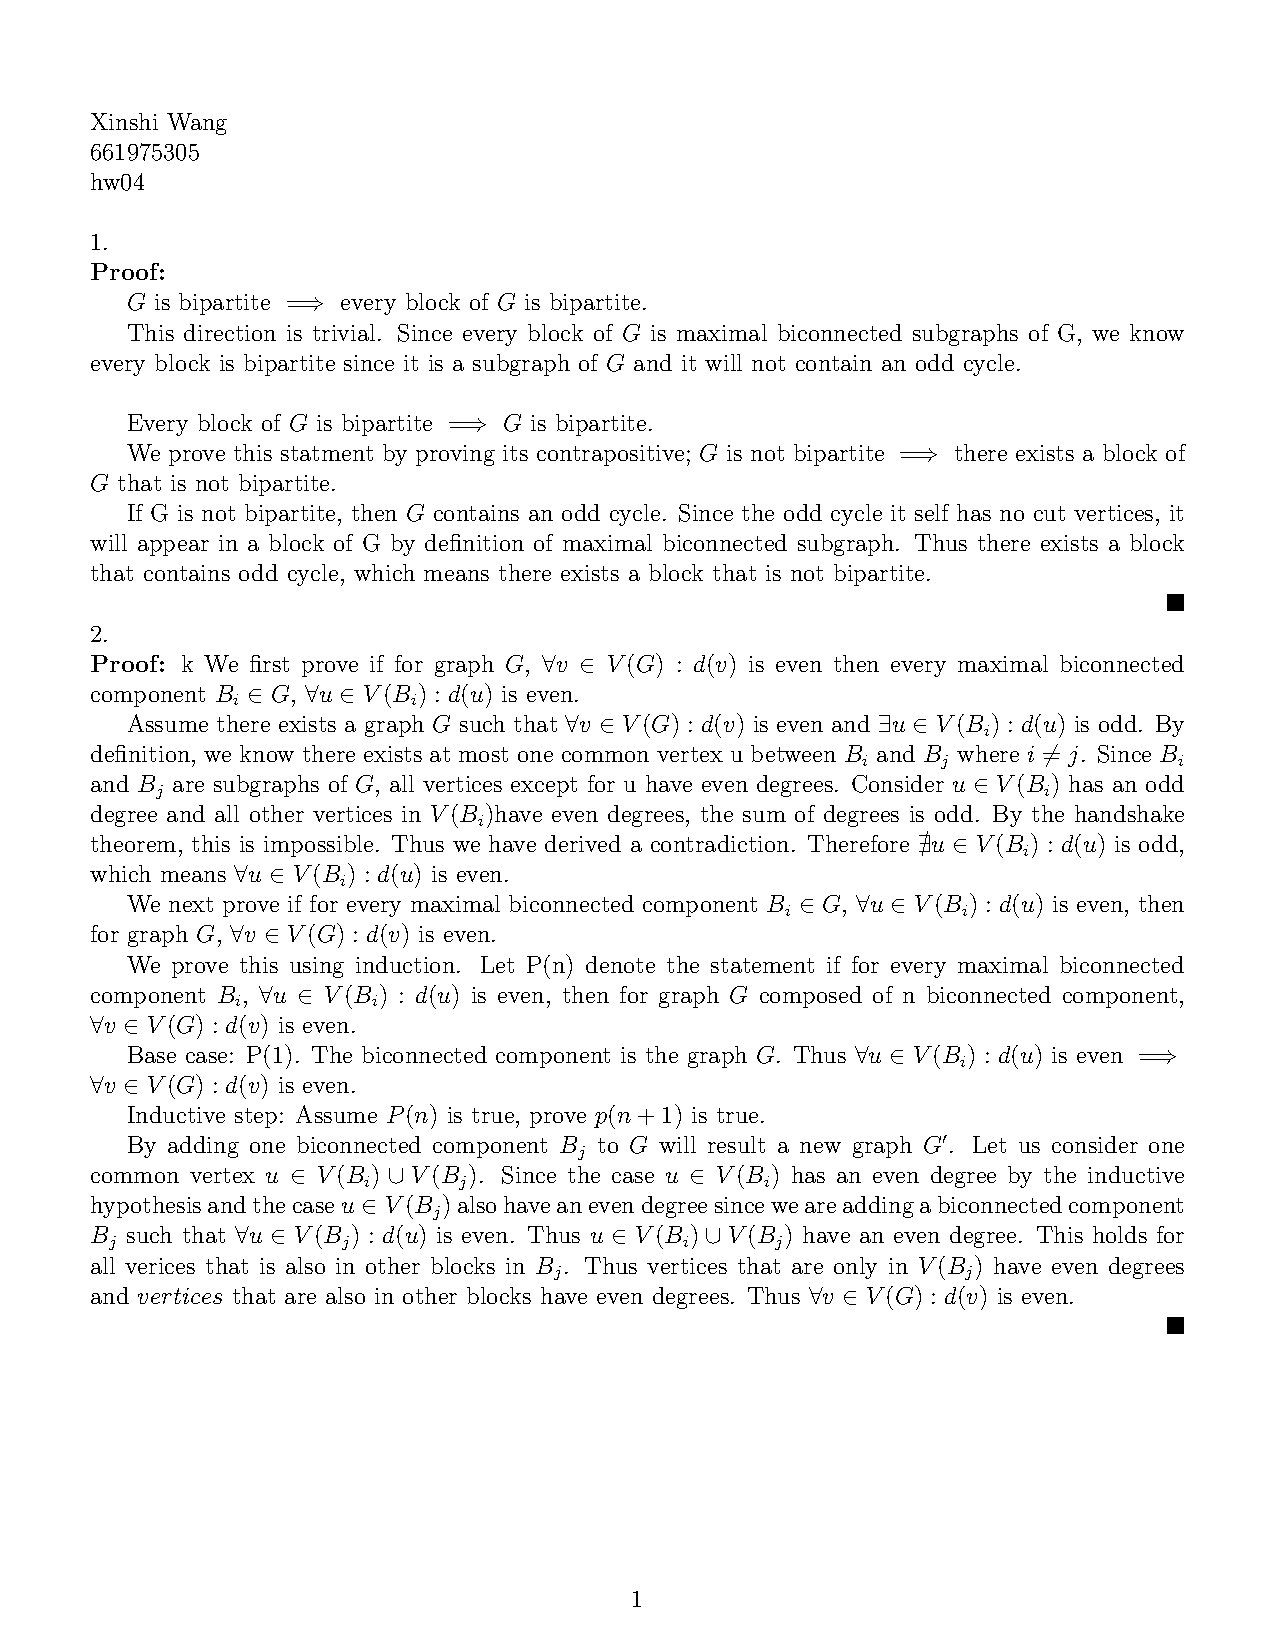
\includegraphics[scale = 0.2]{"C:/Users/Micha/OneDrive - Rensselaer Polytechnic Institute/MATH2400/pictures/hw4.jpg"}
%Problem 2
\item (20 points)  Consider the initial-value problem
\begin{equation*}
t^2y''-ty'+5y=0, \quad y(1)=3, \; y'(1) = -1.
\end{equation*}
\benum
\item Find a fundamental set of solutions in real form.

Assume the solution has the form $y = t^r$. Then
$$y' = rt^{r-1}$$ $$y''= r(r-1)t^{r-2}$$

Then we have 
$$ty' = rt^{r}$$
$$t^2y'' = r(r-1)t^r$$

Then we have 
$$r(r-1)t^r - rt^{r} + 5t^{r} = 0$$
$$r^2-2r+5 = 0$$

Therefore we have $r = 1 \pm 2i$\\
Thus the general solution is $y(t) = t[C_1cos(2ln(t))+C_2sin(2ln(t))]$
\item Find the solution of the initial-value problem.
We take the derivative of $y(t)$
$$y'(t) = [C_1cos(2 \ln (t))+C_2sin(2 \ln (t))] + 2[C_2cos(2ln(t))-C_1sin(2ln(t)))]$$

Then from our IC we have
\begin{equation*}
	\begin{cases}
		C_1 &= 3\\
		C_1 + 2C_2 &= -1\\
	\end{cases}
\end{equation*}
Thus $C_1 = 3$ and $C_2 = -2$.
Then we have the solution: $y(t) = t[3cos(2ln(t))-2sin(2ln(t))]$
\item What is the interval of validity of the solution?

$t > 0$
\eenum



\end{enumerate}

\end{document}